\section{Idea \& Implementation}

\subsection{Idea}

\noindent The main idea can be split into the following steps (which also are
the states of the main controller, \hl{SwarmRobotics.lua}).

\begin{enumerate}
    \item Initialization
    \item Robots split into rooms by going to the nearest room. It does not
    ensure that a robot of each type will be in each room (see Analysis \&
    Problems section).
    \item Go towards target: light source for light robots, and door step for
    ground robots. Compute the 3 values to evaluate the room.
    \item Robots go towards farther robots in order to exit the current room.
    They group themselves inside the central room and share partial scores to
    obtain total score for their assignated room. Once total scores are computed,
    they can be shared to decide which is the best one.
    \item Go towards the best detected room.
\end{enumerate}

\subsection{Implementation details}


\subsubsection{MoveIntoRoom}

The \hl{MoveIntoRoom} state machine has for purpose to let robots go towards
a room and detect when the robot is inside said room. First, the robot is
attracted by the door associated with the room. When the robot is close enough
to the door (1st threshold), then it is attracted by elements inside the room
(objects and light source). Once a 2nd threshold has been reached, the robot is
considered inside the room.

\subsection{Main steps}

\begin{figure}[h!]
        \centering
        \begin{subfigure}[b]{0.5\textwidth}
            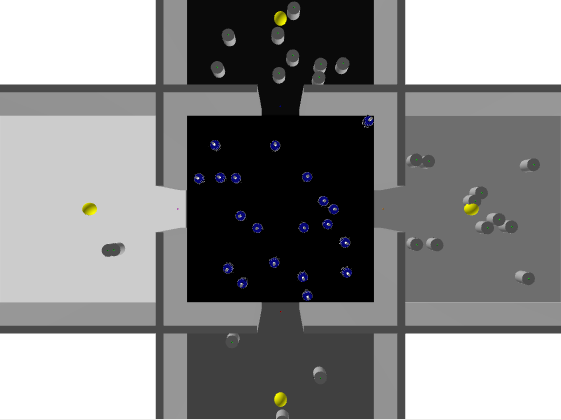
\includegraphics[width=\textwidth]{images/1_start.png}
            \caption{Start}
        \end{subfigure}%
        ~
        \begin{subfigure}[b]{0.5\textwidth}
            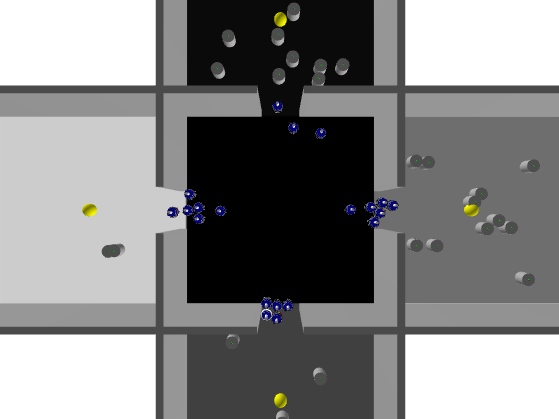
\includegraphics[width=\textwidth]{images/2_split.png}
            \caption{Split}
        \end{subfigure}
        \hfill
        \begin{subfigure}[b]{0.5\textwidth}
            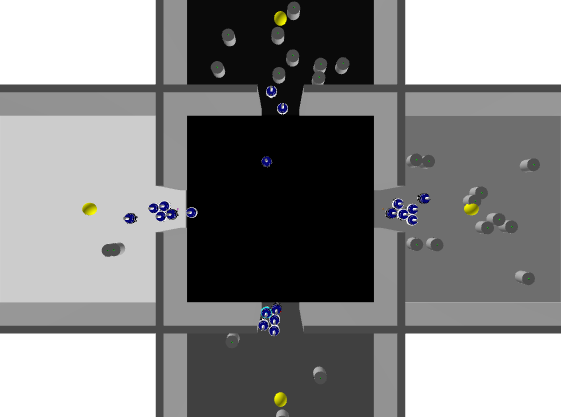
\includegraphics[width=\textwidth]{images/3_evaluate.png}
            \caption{Room evaluation}
        \end{subfigure}%
        ~
        \begin{subfigure}[b]{0.5\textwidth}
            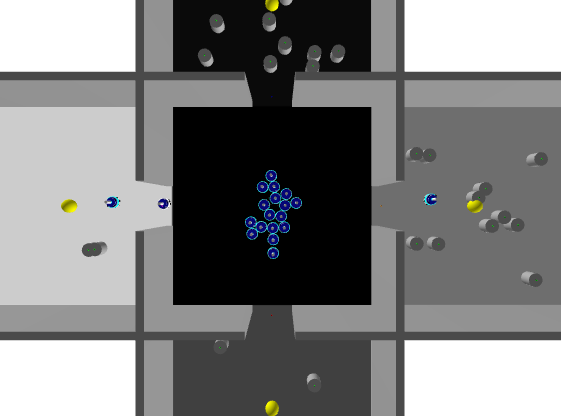
\includegraphics[width=\textwidth]{images/4_sync.png}
            \caption{Gathering \& scores sync}
        \end{subfigure}
        \hfill
        \begin{subfigure}[b]{0.5\textwidth}
            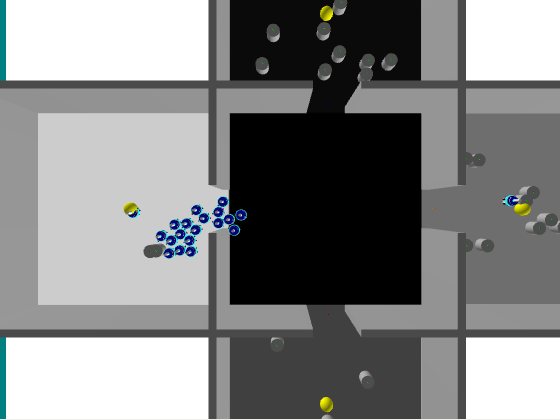
\includegraphics[width=\textwidth]{images/5_best.png}
            \caption{Go to best room}
        \end{subfigure}
        \caption{Main steps}\label{fig:steps}
\end{figure}

% TODO screenshots steps
\newpage
